%1881
\newpage
\subsection{例題4-10 ゲームの背景や絵を改造してみよう}


\begin{description}
    \item \textgt{\bf  考え方}
\end{description}

ジャンプアップゲーム(jump.hsp)のプログラムで使われている画像を確認してみましょう。

画像を書き換えて、自分だけのゲーム画面を作ることもできます。

\begin{figure}[H]
    \begin{center}
      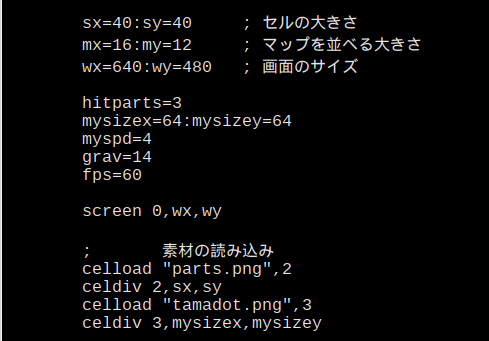
\includegraphics[keepaspectratio]{text04-img/text04-img026.png}
    \end{center}
    \label{fig:prog_menu}
\end{figure}

celload命令で読み込まれているファイルが、ゲームに出てくる画像となります。

操作する主人公は「tamadot.png」という画像です

面を構成するパーツは、「parts.png」という画像にまとめられています。

\begin{figure}[H]
    \begin{center}
      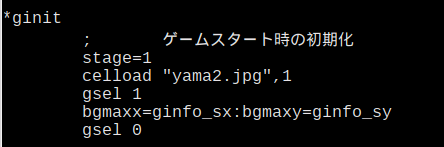
\includegraphics[keepaspectratio,width=10.689cm,height=3.538cm]{text04-img/text04-img027.png}
    \end{center}
    \label{fig:prog_menu}
\end{figure}

また、ゲームの背景は、「yama2.jpg」という画像が使われています。

それぞれが、どんな役割を果たしているか、実際にGIMPなどのツールで確認してみましょう。



\begin{description}
    \item \textgt{\bf 例題4-10 答え}
\end{description}



ジャンプアップゲームの背景は、実は小さな絵を並べて、大きな世界を作っています。

GIMPを使って、ジャンプアップゲームの絵を改造してみましょう。

小さな絵を実際に見て改造をしてみましょう。以前にやった手順を覚えていますか?

「parts.png」アイコンの右クリックメニューから「GNU Image Manipulation Program」をクリックして、GIMPツールを起動させましょう。


\begin{figure}[H]
    \begin{center}
      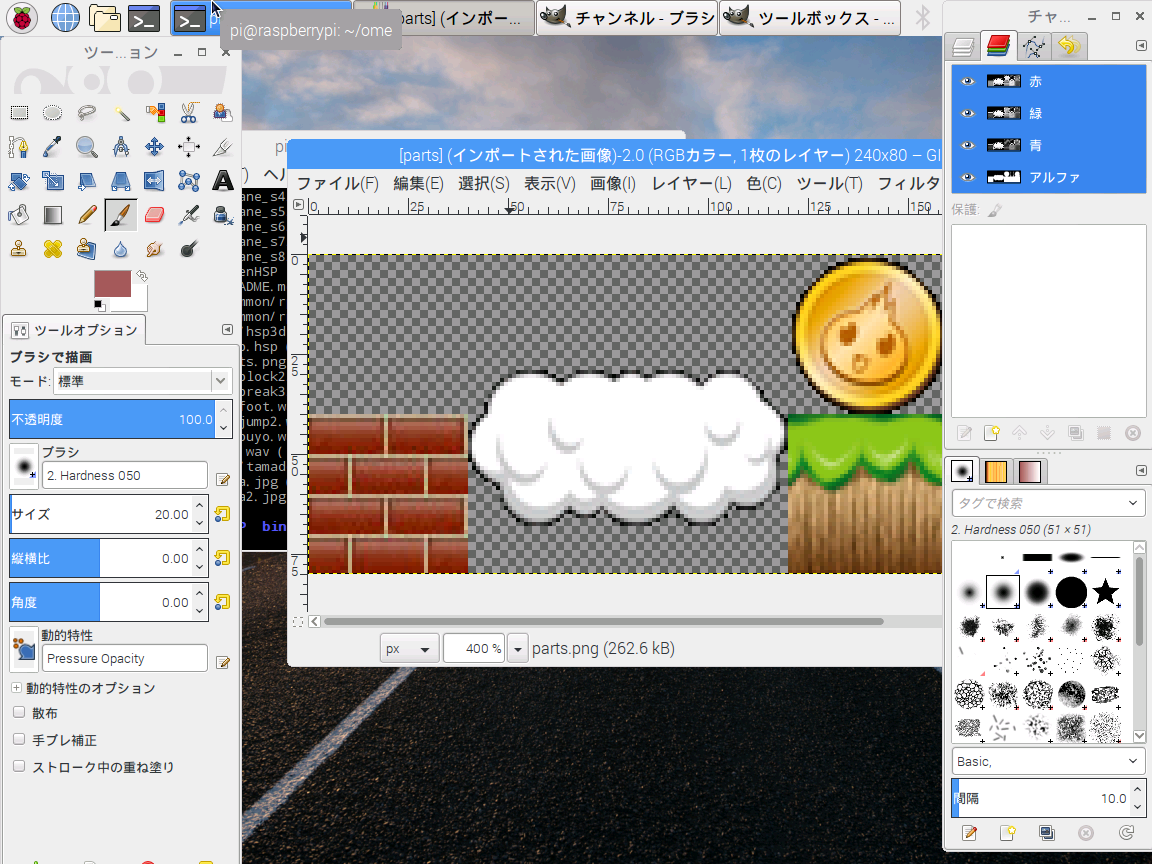
\includegraphics[keepaspectratio,width=12.065cm,height=9.049cm]{text04-img/text04-img029.png}
      \caption{parts.pngを修正している画面}
    \end{center}
    \label{fig:prog_menu}
\end{figure}

パレットで色を選んで、鉛筆のツールで絵を書いていきます。


\begin{figure}[H]
    \begin{center}
      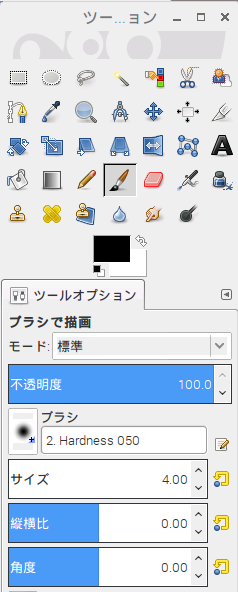
\includegraphics[keepaspectratio,width=4.075cm,height=10.16cm]{text04-img/text04-img030.png}
    \end{center}
    \label{fig:prog_menu}
\end{figure}


元の絵があった部分を書き換えて他の絵柄にしてみましょう。

画像が小さい場合は、画像の下にある「100\%」の右側にあるボタンを押して、「400\%」「800\%」などを選ぶと拡大されます。

絵を修正する時には、ツールアイコンの中から「ブラシ」を選択して、サイズを4〜6くらいの数字に変えてから絵の上で、マウスボタンを押しながら動かして色を置きます。


色を変更する場合は、ツールパレットの描画色をクリックして、「描画色の変更」ダイアログを出してから好きな色を選びます。

\begin{figure}[H]
    \begin{center}
      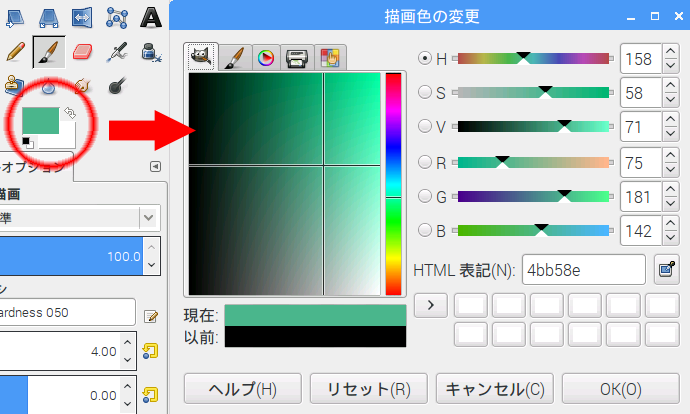
\includegraphics[keepaspectratio,width=10.993cm,height=6.588cm]{text04-img/text04-img031.png}
    \end{center}
    \label{fig:prog_menu}
\end{figure}

元の絵を書き換えたら、ファイル→「parts.pngに上書きエクスポート」を選んで保存します。

背景画像は、縦長のもので「yama2.jpg」として保存されています。変更した画像でゲームを動かしてみましょう。


\begin{figure}[H]
    \begin{center}
      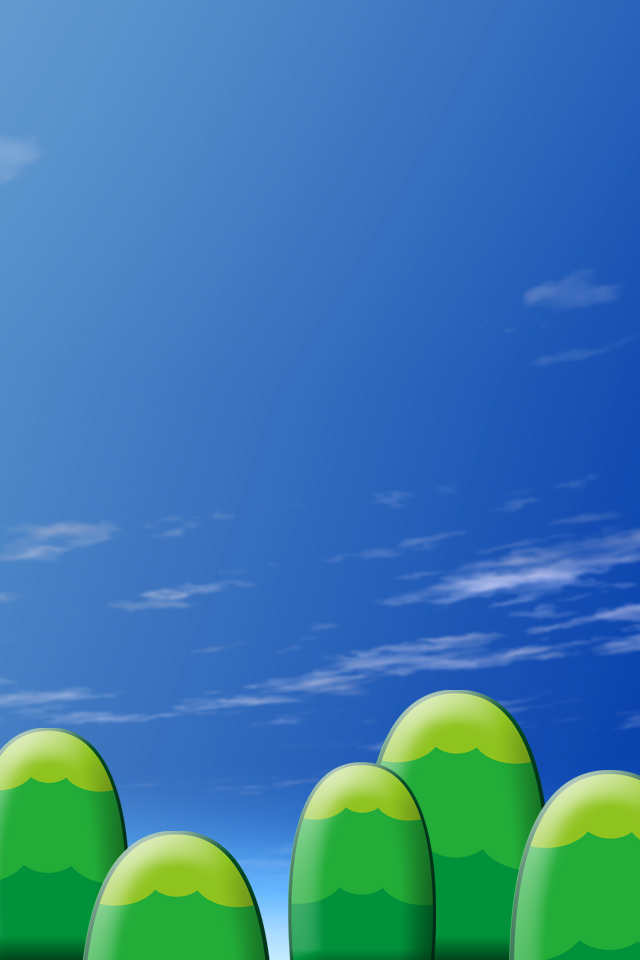
\includegraphics[keepaspectratio,width=8.546cm,height=12.804cm]{text04-img/text04-img032.jpg}
    \end{center}
    \label{fig:prog_menu}
\end{figure}

[F5]キーを押して実行して変わっていれば成功です。

改造ができたらTAや周りの友達にも見せてあげましょう。

%2038
